% mn2esample.tex
%
% v2.1 released 22nd May 2002 (G. Hutton)
%

\documentclass[useAMS,usenatbib]{mn2e}

\usepackage[pdftex]{graphicx}
\usepackage{verbatim}
\usepackage{natbib}
\usepackage{amsmath}
\usepackage{color}
\usepackage{deluxetable}
\usepackage{enumerate}
\usepackage{comment}
\usepackage{hyperref}
\bibliographystyle{mn2e}

%%%%% AUTHORS -- PLACE YOUR OWN MACROS HERE %%%%%

%\input blazarenv_macros.tex	
\newcommand{\mnras}{MNRAS}
\newcommand{\apj}{ApJ}
\newcommand{\aj}{AJ}
\newcommand{\apjl}{ApJL}
\newcommand{\apjs}{ApJS}
\newcommand{\aap}{A\&A}
\newcommand{\araa}{ARA\&A}
\newcommand{\fcp}{FCP}
\newcommand{\dcoadd}{$\Delta_{coadd}$}
\newcommand{\mr}{$M_r$}
\newcommand{\rfifty}{$R_{50}$}
\newcommand{\redshift}{$z$}

\renewcommand{\thefootnote}{\fnsymbol{footnote}}

%%%%%%%%%%%%%%%%%%%%%%%%%%%%%%%%%%%%%%%%%%%%%%%%

\title[GZ2 gallery]{Galaxy~Zoo~2: gallery of images for robust classifications}
\author[Willett et al.]{
  \parbox[t]{16cm}{
  Kyle W. Willett $^{1}$\thanks{E-mail: willett@physics.umn.edu},
  Chris J. Lintott$^{2}$,
  Steven P. Bamford$^{3}$,
  Karen L. Masters$^{4}$,
  Brooke D. Simmons$^{2}$,
  Kevin Schawinski$^{5}$,
  Lucy Fortson$^{1}$,
  Robert J. Simpson$^{2}$,
  Ramin A. Skibba$^{6}$,
  Edward M. Edmondson$^{4}$,
  Arfon M. Smith$^{2,7}$\\
  }\\
$^{1}$University of Minnesota, USA \\
$^{2}$University of Oxford, UK \\
$^{3}$University of Nottingham, UK \\
$^{4}$University of Portsmouth, UK \\
$^{5}$ETH, Z\"urich, Switzerland \\
$^{6}$University of California San Diego, USA \\
$^{7}$Adler Planetarium, USA \\
}

\begin{document}

\date{Accepted 1988 December 15. Received 1988 December 14; in original form 1988 October 11}

\pagerange{\pageref{firstpage}--\pageref{lastpage}} \pubyear{2012}

\maketitle

\label{firstpage}

\begin{abstract}
Gallery of example images for the accompanying Galaxy~Zoo~2 data release paper. 
\end{abstract}

\begin{keywords}
galaxies
\end{keywords}

\newpage
\clearpage
\begin{figure*}
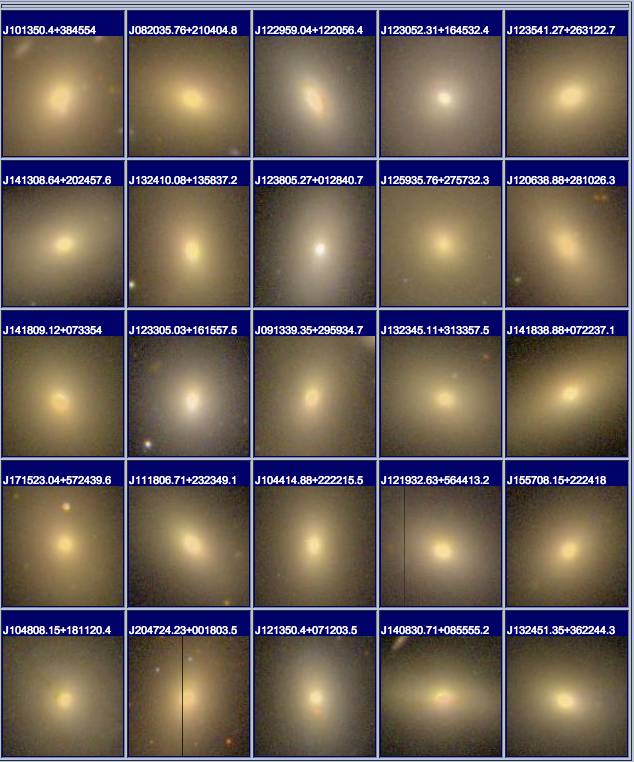
\includegraphics[angle=0,width=7.0in]{figures/gallery/smooth.png}
\caption{Example {\it gri} cutout images for galaxies identified as ``smooth'' (Task 01, Answer 01) from the GZ2 clean, debiased sample as set by flags in the table. Cutout images are from the SDSS DR7 Image List Tool (\url{http://cas.sdss.org/dr7/en/tools/chart/list.asp}).  
\label{fig1}}
\end{figure*}

\newpage
\clearpage
\begin{figure*}
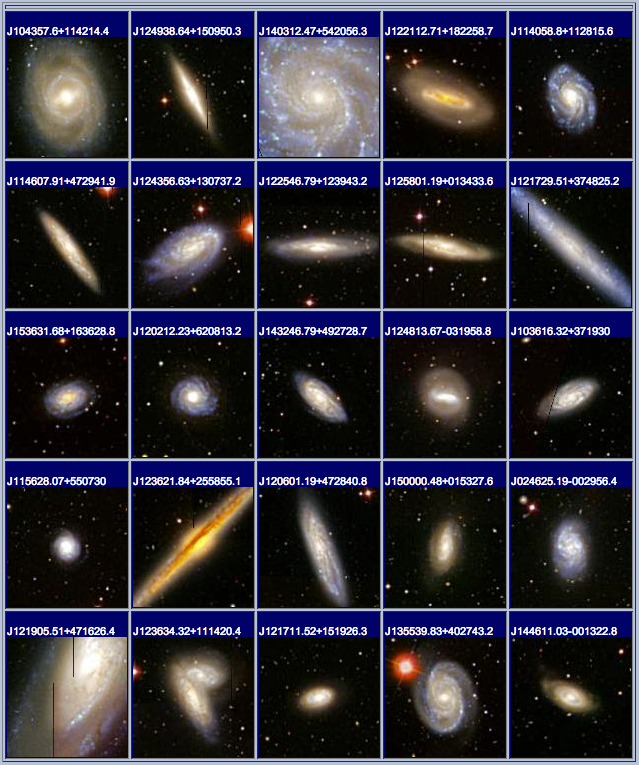
\includegraphics[angle=0,width=7.0in]{figures/gallery/features.png}
\caption{Example $gri$ cutout images for galaxies identified as ``features or disk'' (Task 01, Answer 02) from the GZ2 clean, debiased sample. Format is the same as Figure~\ref{fig1}.}
\end{figure*}

\newpage
\clearpage
\begin{figure*}
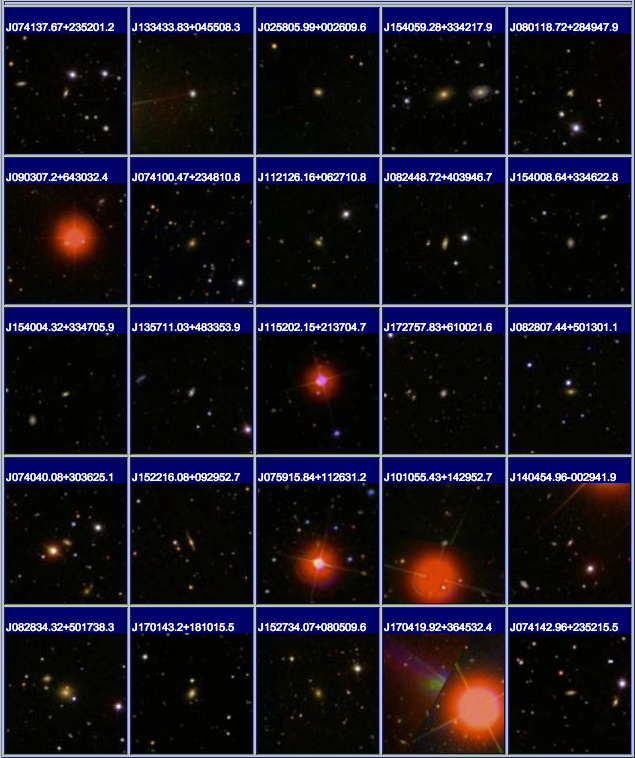
\includegraphics[angle=0,width=7.0in]{figures/gallery/artifact.png}
\caption{Example $gri$ cutout images for objects identified as ``star or artifact'' (Task 01, Answer 03) from the GZ2 clean, debiased sample. Format is the same as Figure~\ref{fig1}.}
\end{figure*}

\newpage
\clearpage
\begin{figure*}
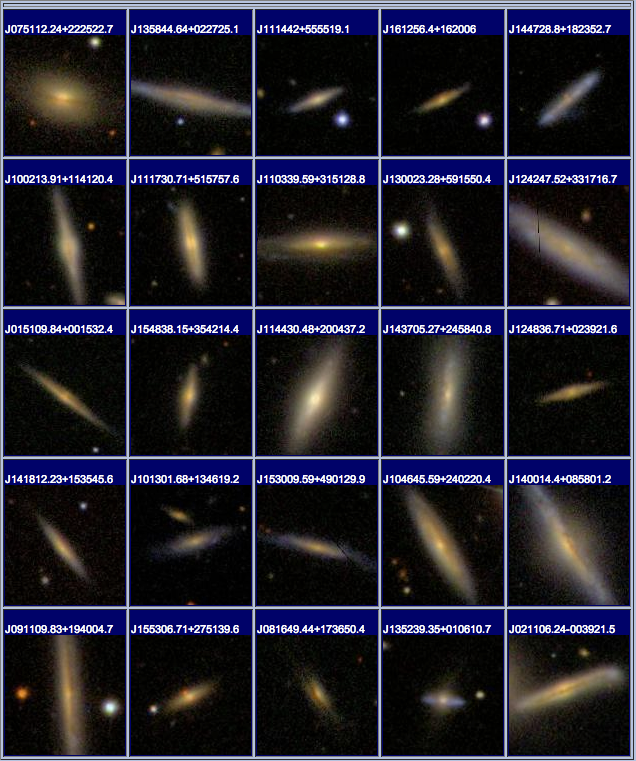
\includegraphics[angle=0,width=7.0in]{figures/gallery/edgeon.png}
\caption{Example $gri$ cutout images for galaxies identified as ``edge-on'' (Task 02, Answer 04) from the GZ2 clean, debiased sample. Format is the same as Figure~\ref{fig1}.}
\end{figure*}

\newpage
\clearpage
\begin{figure*}
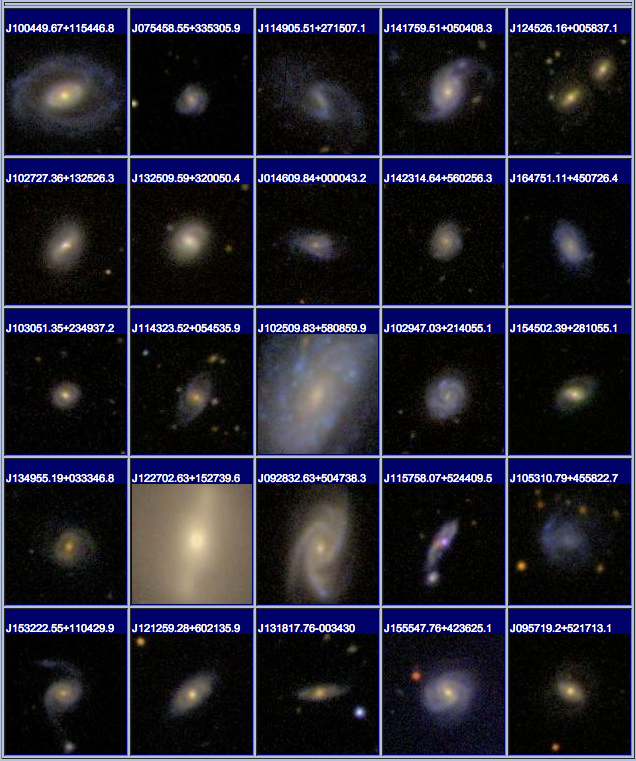
\includegraphics[angle=0,width=7.0in]{figures/gallery/notedgeon.png}
\caption{Example $gri$ cutout images for galaxies identified as ``not edge-on'' (Task 02, Answer 05) from the GZ2 clean, debiased sample. Format is the same as Figure~\ref{fig1}.}
\end{figure*}

\newpage
\clearpage
\begin{figure*}
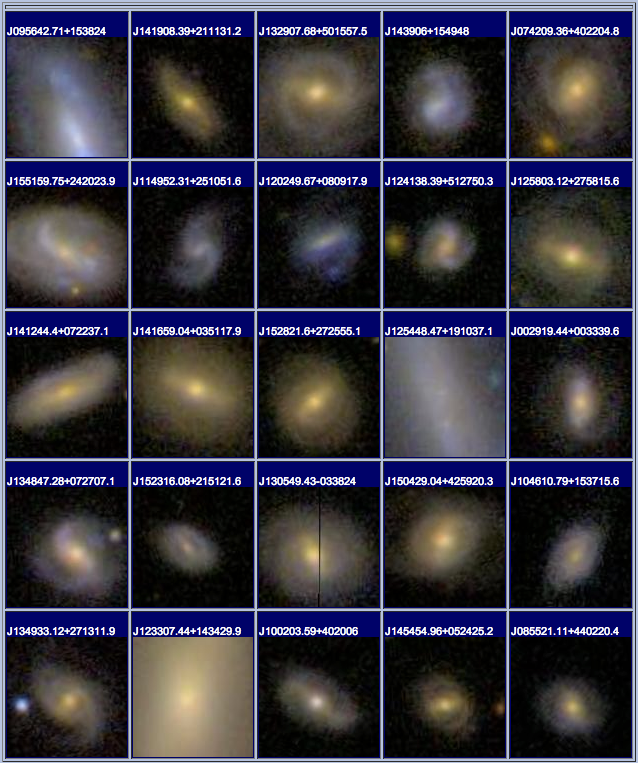
\includegraphics[angle=0,width=7.0in]{figures/gallery/bar.png}
\caption{Example $gri$ cutout images for galaxies identified as ``bar'' (Task 03, Answer 06) from the GZ2 clean, debiased sample. Format is the same as Figure~\ref{fig1}.}
\end{figure*}

\newpage
\clearpage
\begin{figure*}
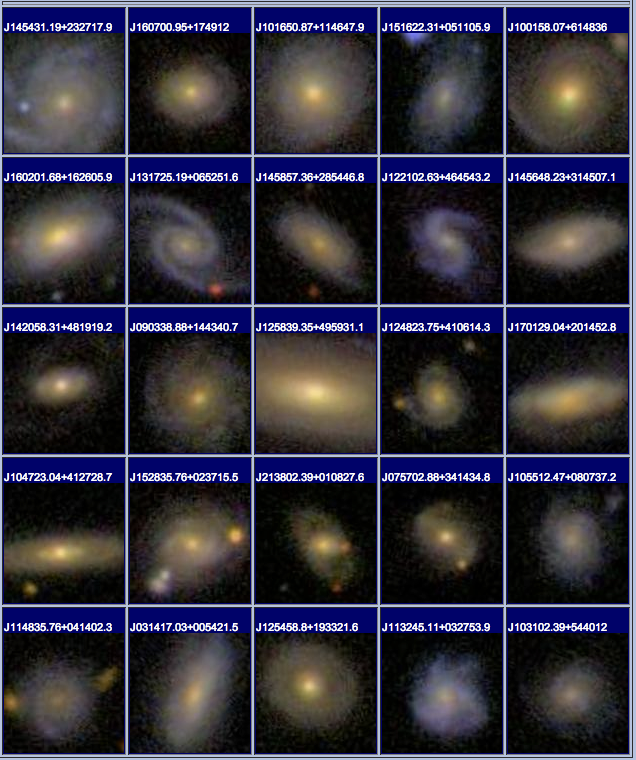
\includegraphics[angle=0,width=7.0in]{figures/gallery/nobar.png}
\caption{Example $gri$ cutout images for galaxies identified as ``no bar'' (Task 03, Answer 07) from the GZ2 clean, debiased sample. Format is the same as Figure~\ref{fig1}.}
\end{figure*}

\newpage
\clearpage
\begin{figure*}
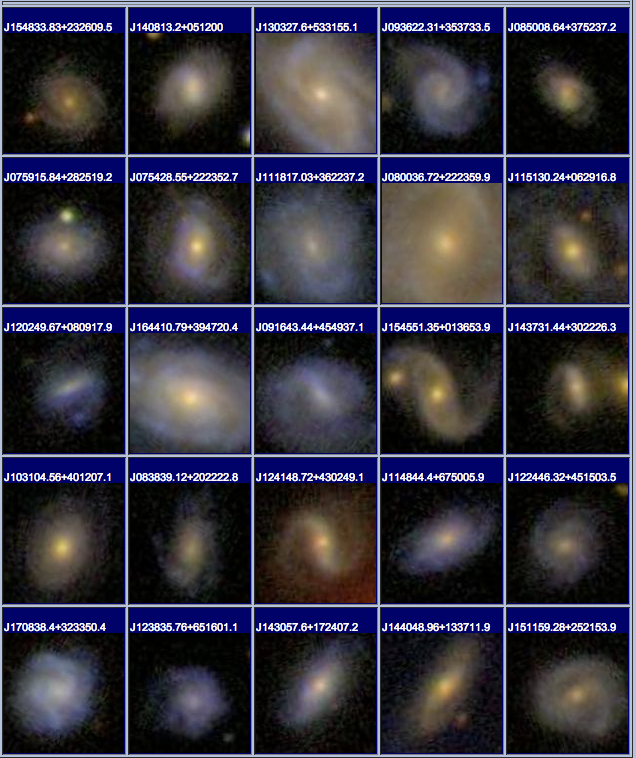
\includegraphics[angle=0,width=7.0in]{figures/gallery/spiral.png}
\caption{Example $gri$ cutout images for galaxies identified as having ``spiral'' structure (Task 04, Answer 08) from the GZ2 clean, debiased sample. Format is the same as Figure~\ref{fig1}.}
\end{figure*}

\newpage
\clearpage
\begin{figure*}
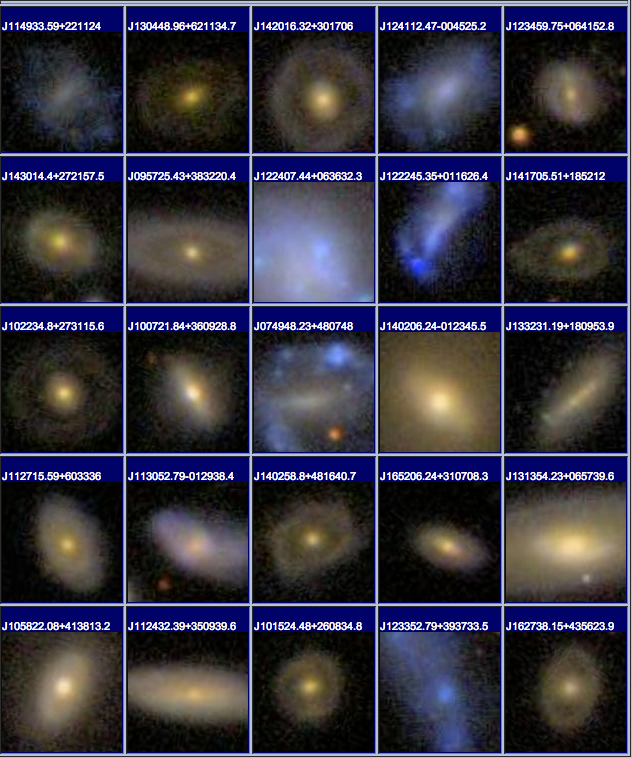
\includegraphics[angle=0,width=7.0in]{figures/gallery/nospiral.png}
\caption{Example $gri$ cutout images for galaxies identified as having ``no spiral'' structure (Task 04, Answer 09) from the GZ2 clean, debiased sample. Format is the same as Figure~\ref{fig1}.}
\end{figure*}

\newpage
\clearpage
\begin{figure*}
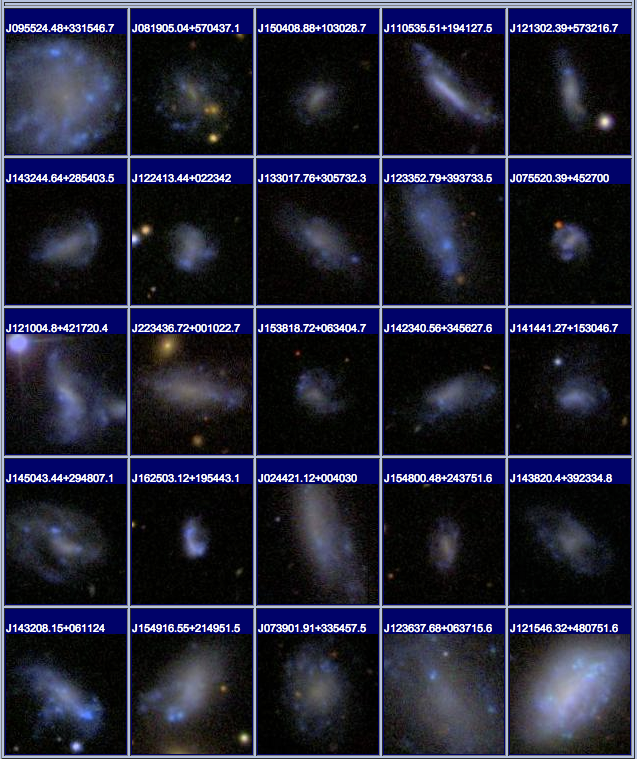
\includegraphics[angle=0,width=7.0in]{figures/gallery/nobulge.png}
\caption{Example $gri$ cutout images for galaxies identified as having ``no bulge'' (Task 05, Answer 10) from the GZ2 clean, debiased sample. Format is the same as Figure~\ref{fig1}.}
\end{figure*}

\newpage
\clearpage
\begin{figure*}
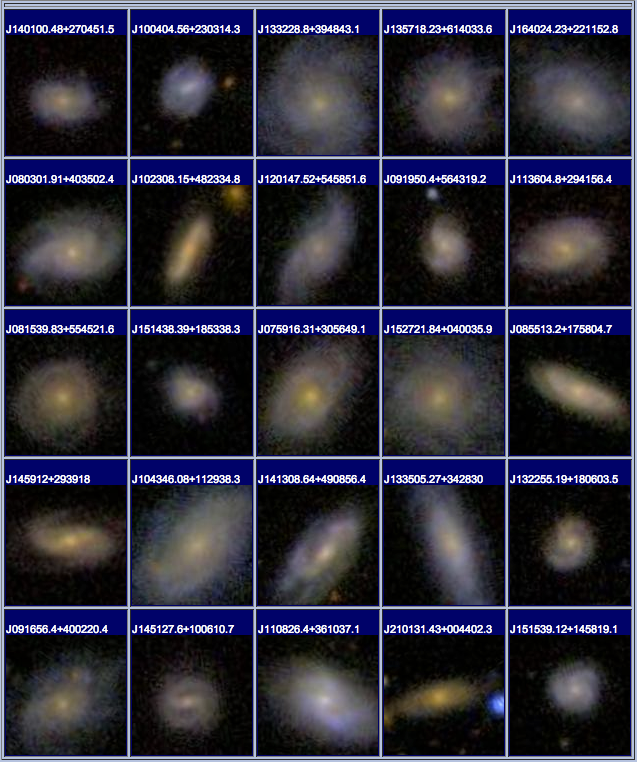
\includegraphics[angle=0,width=7.0in]{figures/gallery/justnoticeable.png}
\caption{Example $gri$ cutout images for galaxies identified as having a ``just noticeable'' bulge (Task 05, Answer 11) from the GZ2 clean, debiased sample. Format is the same as Figure~\ref{fig1}.}
\end{figure*}

\newpage
\clearpage
\begin{figure*}
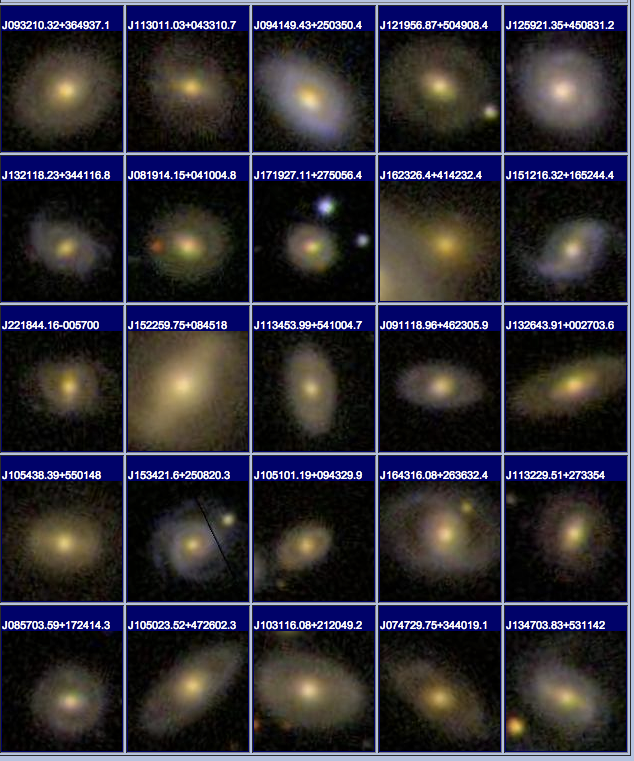
\includegraphics[angle=0,width=7.0in]{figures/gallery/obvious.png}
\caption{Example $gri$ cutout images for galaxies identified as having a ``obvious'' bulge (Task 05, Answer 12) from the GZ2 clean, debiased sample. Format is the same as Figure~\ref{fig1}.}
\end{figure*}

\newpage
\clearpage
\begin{figure*}
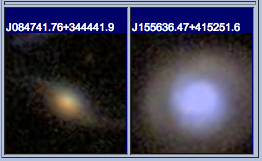
\includegraphics[angle=0,width=7.0in]{figures/gallery/dominant.png}
\caption{Example $gri$ cutout images for galaxies identified as having a ``dominant'' bulge (Task 05, Answer 13) from the GZ2 clean, debiased sample. Format is the same as Figure~\ref{fig1}.}
\end{figure*}

\newpage
\clearpage
\begin{figure*}
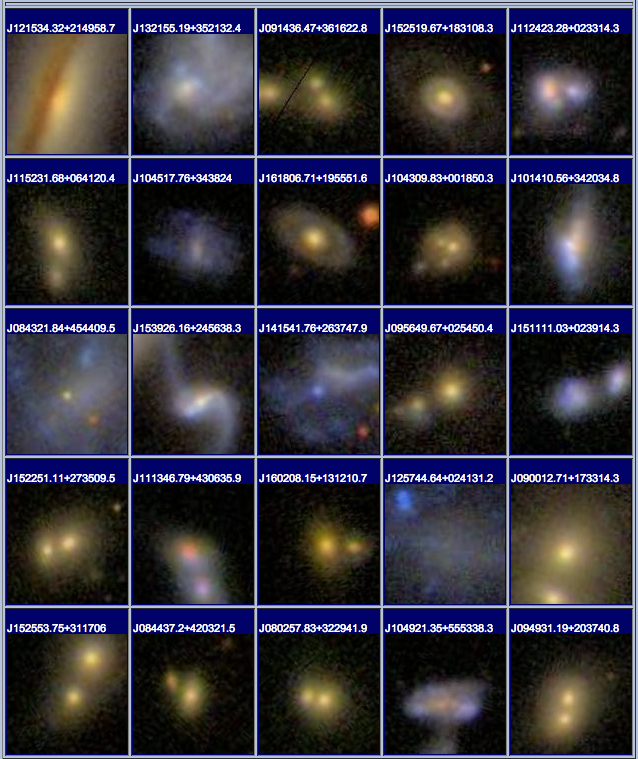
\includegraphics[angle=0,width=7.0in]{figures/gallery/odd.png}
\caption{Example $gri$ cutout images for galaxies identified as ``odd'' (Task 06, Answer 14) from the GZ2 clean, debiased sample. Format is the same as Figure~\ref{fig1}.}
\end{figure*}

\newpage
\clearpage
\begin{figure*}
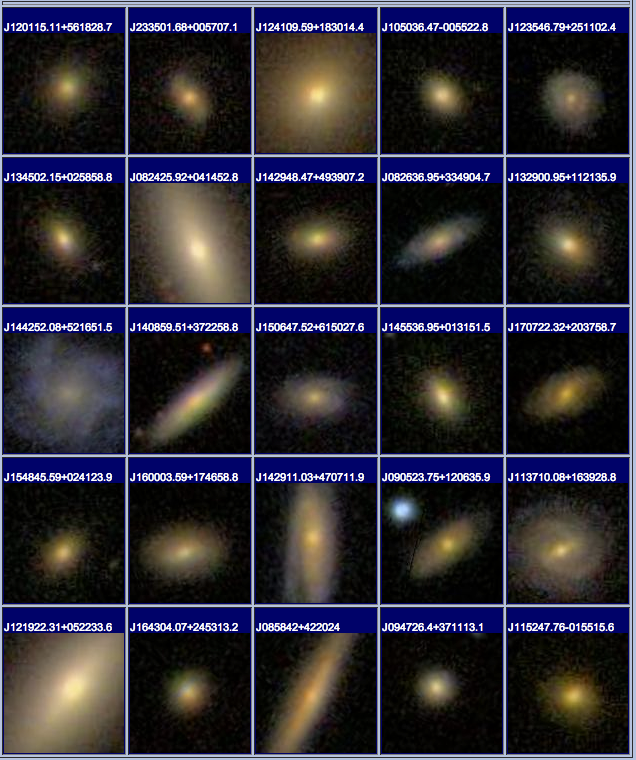
\includegraphics[angle=0,width=7.0in]{figures/gallery/notodd.png}
\caption{Example $gri$ cutout images for galaxies identified as ``not odd'' (Task 06, Answer 15) from the GZ2 clean, debiased sample. Format is the same as Figure~\ref{fig1}.}
\end{figure*}

\newpage
\clearpage
\begin{figure*}
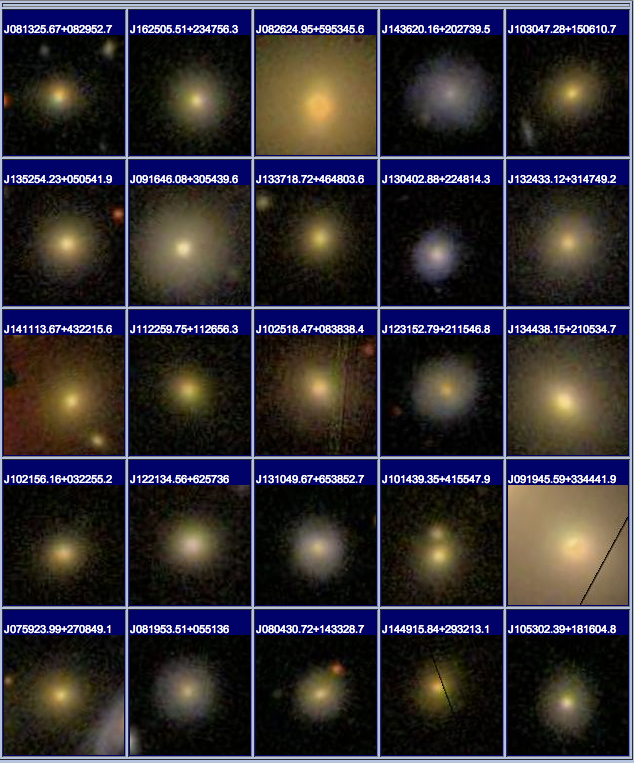
\includegraphics[angle=0,width=7.0in]{figures/gallery/completelyround.png}
\caption{Example $gri$ cutout images for galaxies identified as ``completely round'' (Task 07, Answer 16) from the GZ2 clean, debiased sample. Format is the same as Figure~\ref{fig1}.}
\end{figure*}

\newpage
\clearpage
\begin{figure*}
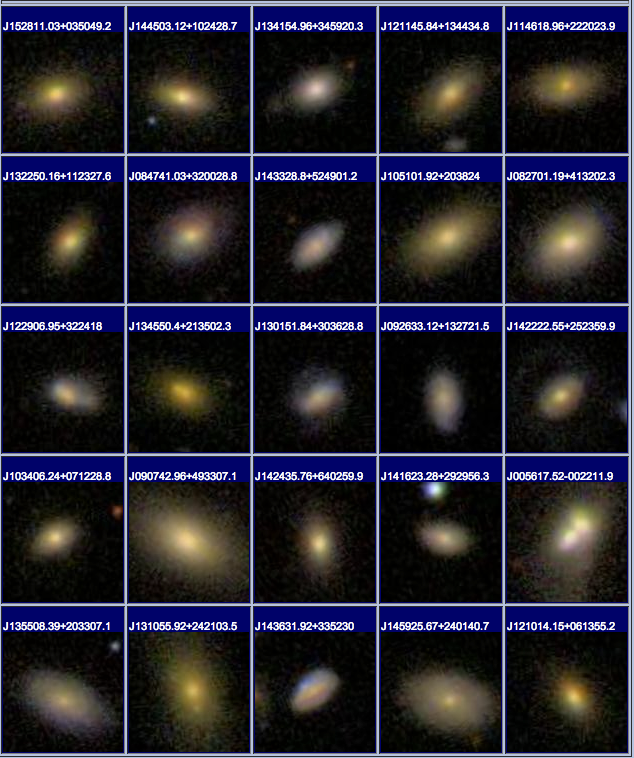
\includegraphics[angle=0,width=7.0in]{figures/gallery/inbetween.png}
\caption{Example $gri$ cutout images for galaxies identified as ``in between'' (Task 07, Answer 17) from the GZ2 clean, debiased sample. Format is the same as Figure~\ref{fig1}.}
\end{figure*}

\newpage
\clearpage
\begin{figure*}
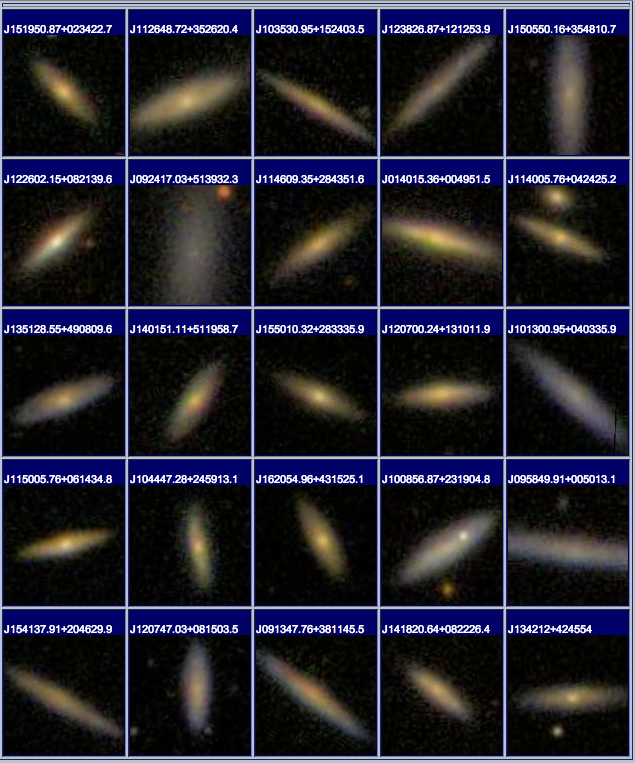
\includegraphics[angle=0,width=7.0in]{figures/gallery/cigarshaped.png}
\caption{Example $gri$ cutout images for galaxies identified as ``cigar shaped'' (Task 07, Answer 18) from the GZ2 clean, debiased sample. Format is the same as Figure~\ref{fig1}.}
\end{figure*}

\newpage
\clearpage
\begin{figure*}
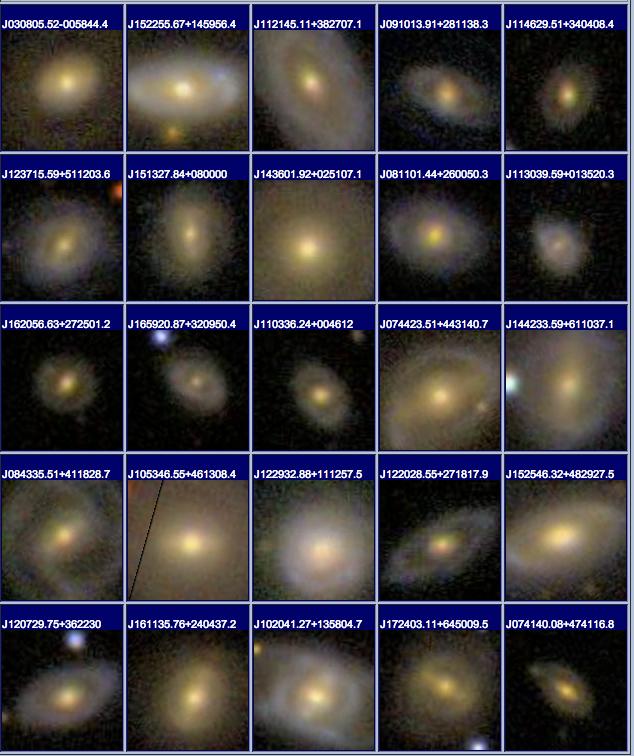
\includegraphics[angle=0,width=7.0in]{figures/gallery/ring.png}
\caption{Example $gri$ cutout images for galaxies identified as ``ring'' (Task 08, Answer 19) from the GZ2 clean, debiased sample. Format is the same as Figure~\ref{fig1}.}
\end{figure*}

\newpage
\clearpage
\begin{figure*}
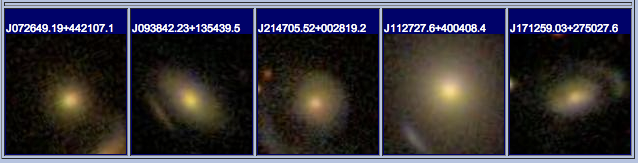
\includegraphics[angle=0,width=7.0in]{figures/gallery/lens.png}
\caption{Example $gri$ cutout images for galaxies identified as ``lens or arc'' (Task 08, Answer 20) from the GZ2 clean, debiased sample. Format is the same as Figure~\ref{fig1}.}
\end{figure*}

\newpage
\clearpage
\begin{figure*}
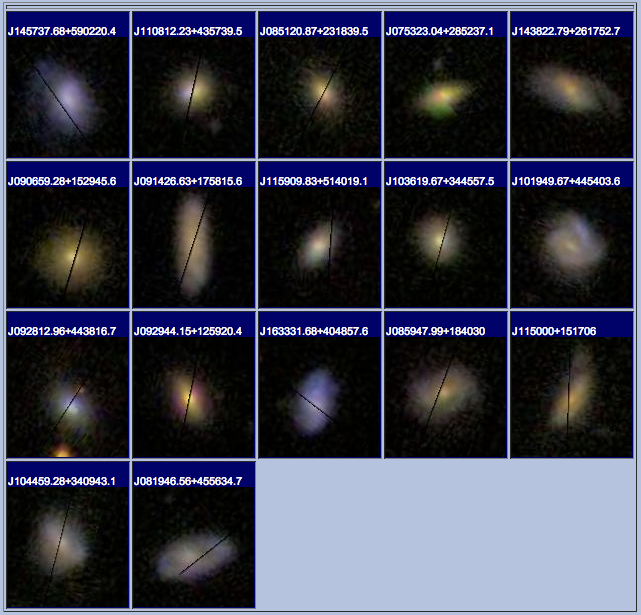
\includegraphics[angle=0,width=7.0in]{figures/gallery/disturbed.png}
\caption{Example $gri$ cutout images for galaxies identified as ``disturbed'' (Task 08, Answer 21) from the GZ2 clean, debiased sample. Format is the same as Figure~\ref{fig1}.}
\end{figure*}

\newpage
\clearpage
\begin{figure*}
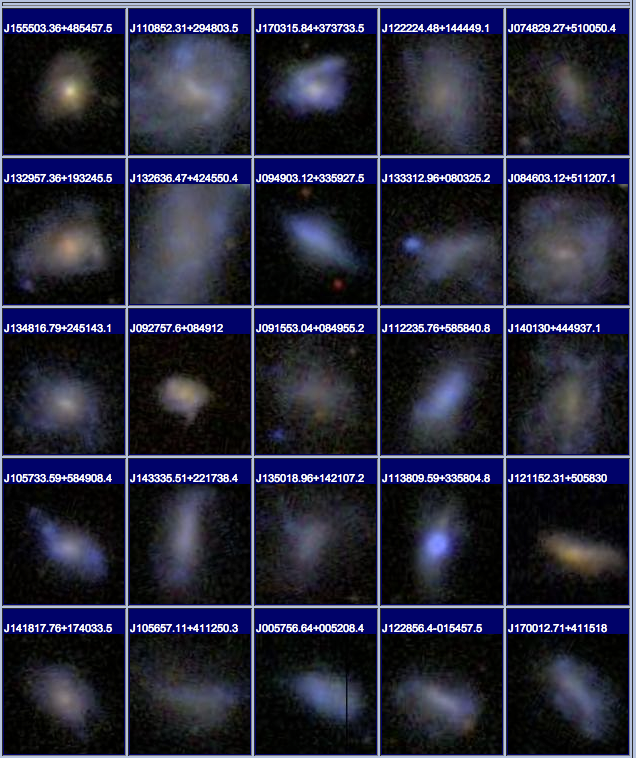
\includegraphics[angle=0,width=7.0in]{figures/gallery/irregular.png}
\caption{Example $gri$ cutout images for galaxies identified as ``irregular'' (Task 08, Answer 22) from the GZ2 clean, debiased sample. Format is the same as Figure~\ref{fig1}.}
\end{figure*}

\newpage
\clearpage
\begin{figure*}
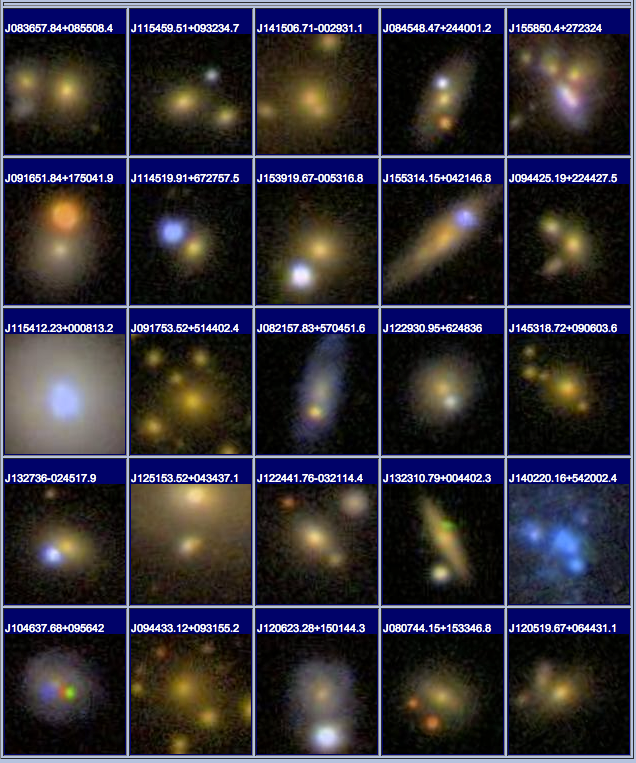
\includegraphics[angle=0,width=7.0in]{figures/gallery/other.png}
\caption{Example $gri$ cutout images for galaxies identified as ``other'' (Task 08, Answer 23) from the GZ2 clean, debiased sample. Format is the same as Figure~\ref{fig1}.}
\end{figure*}

\newpage
\clearpage
\begin{figure*}
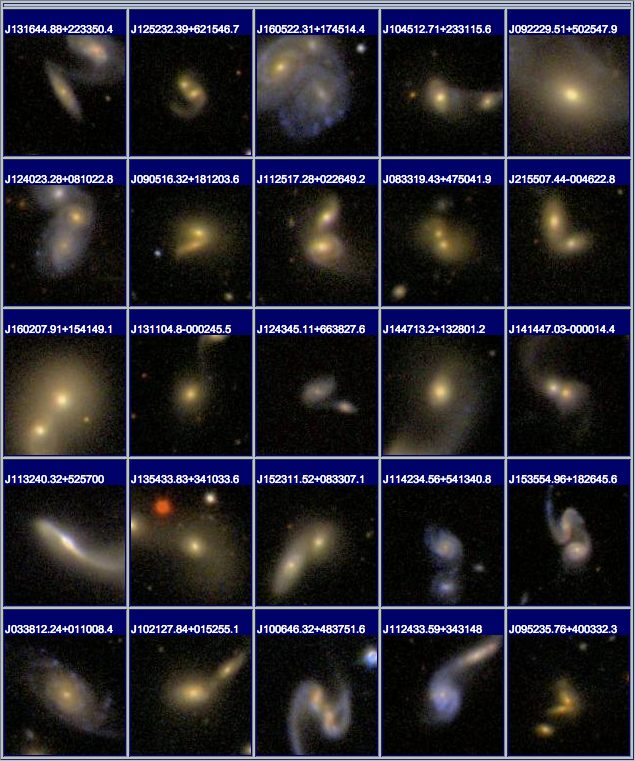
\includegraphics[angle=0,width=7.0in]{figures/gallery/merger.png}
\caption{Example $gri$ cutout images for galaxies identified as ``merger'' (Task 08, Answer 24) from the GZ2 clean, debiased sample. Format is the same as Figure~\ref{fig1}.}
\end{figure*}

\newpage
\clearpage
\begin{figure*}
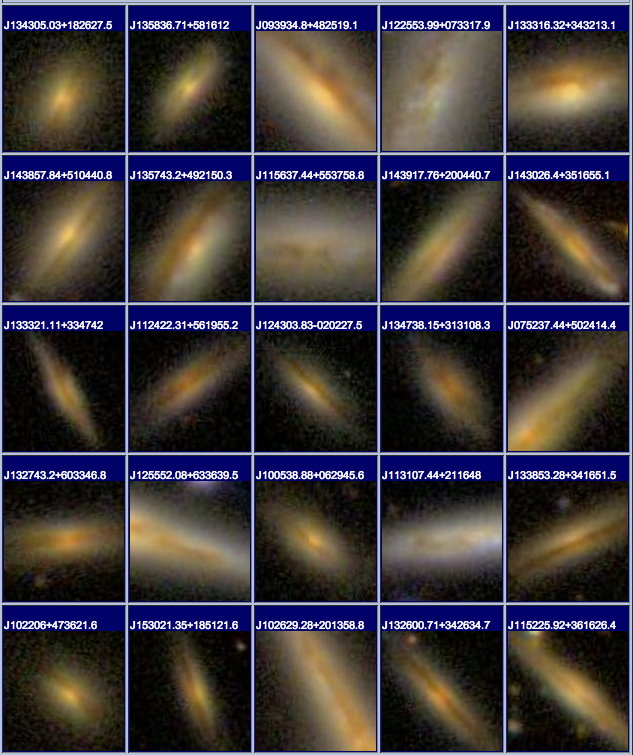
\includegraphics[angle=0,width=7.0in]{figures/gallery/dustlane.png}
\caption{Example $gri$ cutout images for galaxies identified as ``dust lane'' (Task 08, Answer 38) from the GZ2 clean, debiased sample. Format is the same as Figure~\ref{fig1}.}
\end{figure*}

\newpage
\clearpage
\begin{figure*}
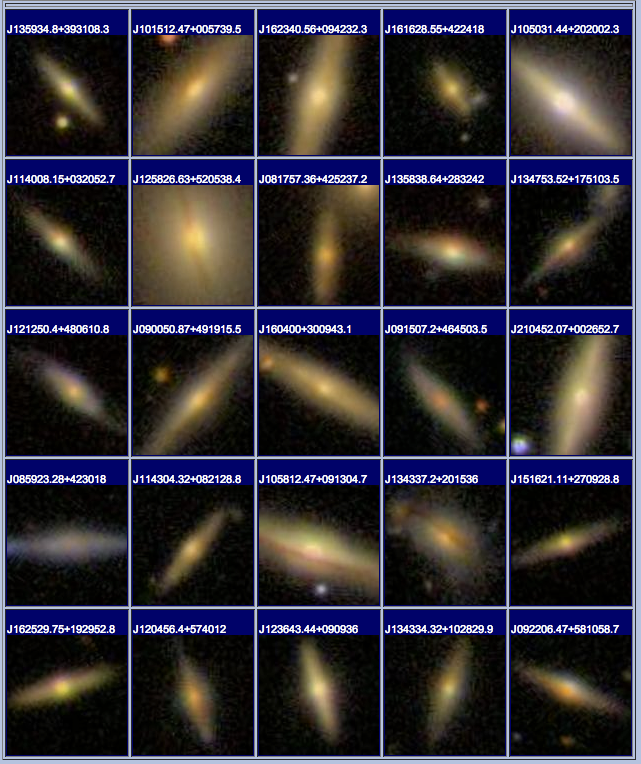
\includegraphics[angle=0,width=7.0in]{figures/gallery/roundedbulge.png}
\caption{Example $gri$ cutout images for galaxies identified as having a ``rounded bulge'' and edge-on (Task 09, Answer 25) from the GZ2 clean, debiased sample. Format is the same as Figure~\ref{fig1}.}
\end{figure*}

\newpage
\clearpage
\begin{figure*}
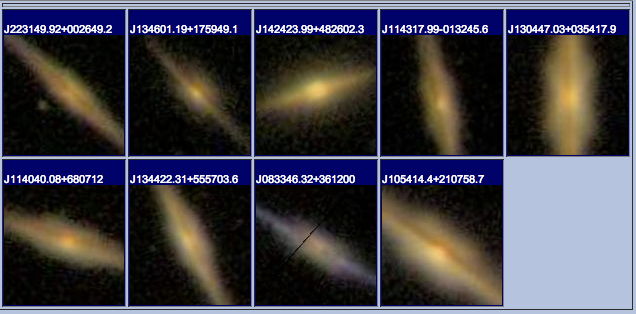
\includegraphics[angle=0,width=7.0in]{figures/gallery/boxybulge.png}
\caption{Example $gri$ cutout images for galaxies identified as having a ``boxy bulge'' and edge-on (Task 09, Answer 26) from the GZ2 clean, debiased sample. Format is the same as Figure~\ref{fig1}.}
\end{figure*}

\newpage
\clearpage
\begin{figure*}
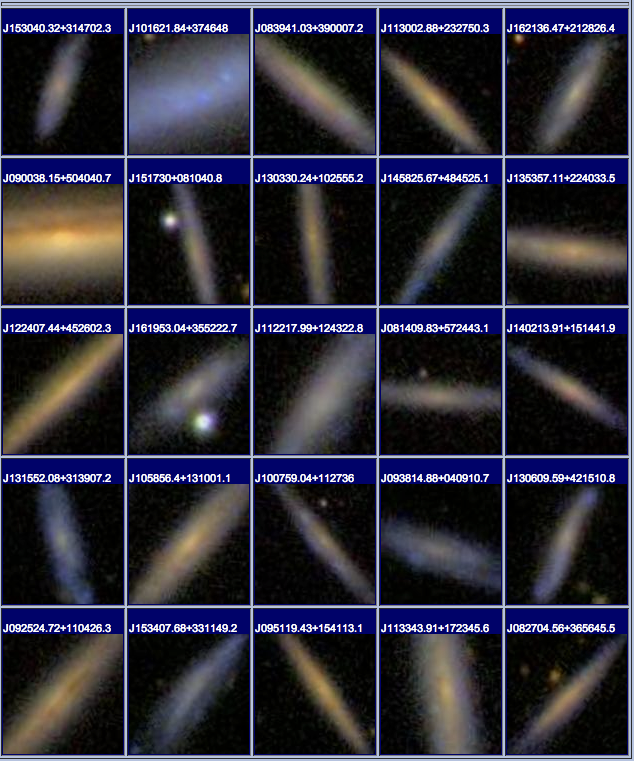
\includegraphics[angle=0,width=7.0in]{figures/gallery/noedgeonbulge.png}
\caption{Example $gri$ cutout images for galaxies identified as having ``no bulge'' and edge-on (Task 09, Answer 27) from the GZ2 clean, debiased sample. Format is the same as Figure~\ref{fig1}.}
\end{figure*}

\newpage
\clearpage
\begin{figure*}
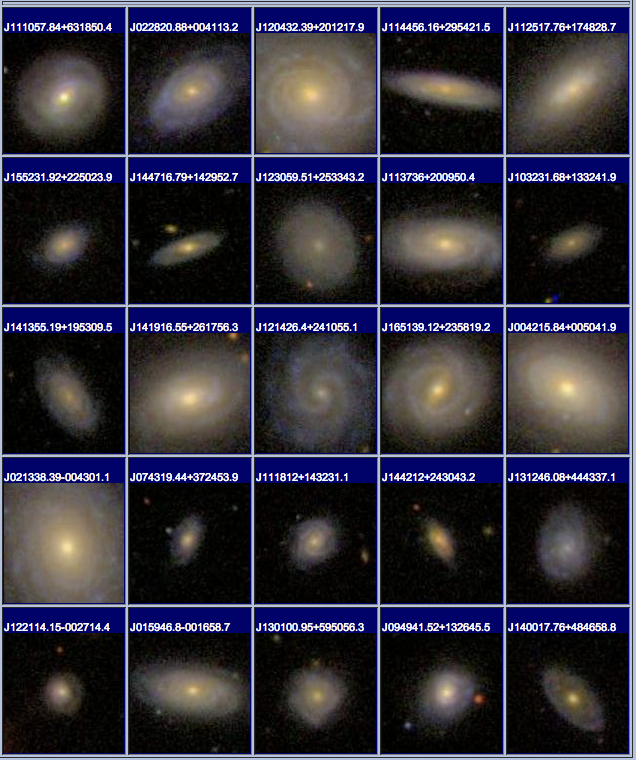
\includegraphics[angle=0,width=7.0in]{figures/gallery/tight.png}
\caption{Example $gri$ cutout images for galaxies identified as having ``tight'' winding spiral arms (Task 10, Answer 28) from the GZ2 clean, debiased sample. Format is the same as Figure~\ref{fig1}.}
\end{figure*}

\newpage
\clearpage
\begin{figure*}
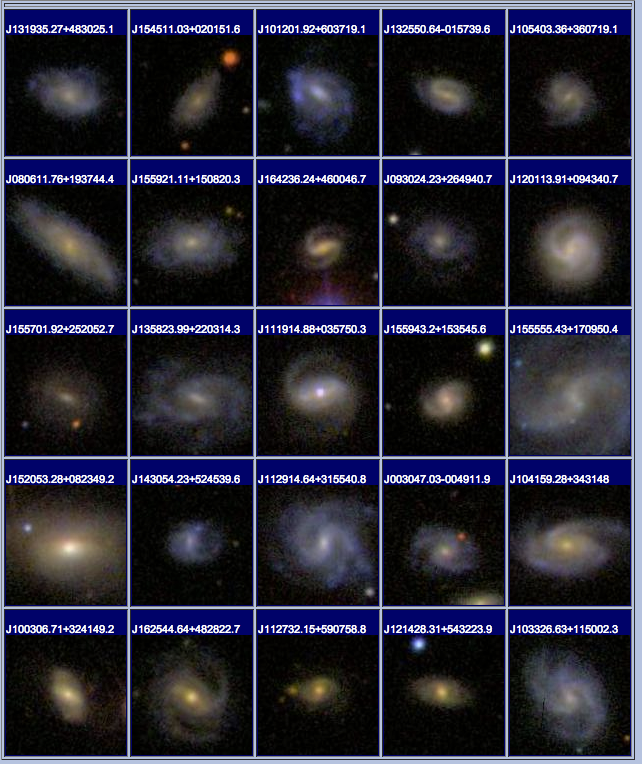
\includegraphics[angle=0,width=7.0in]{figures/gallery/medium.png}
\caption{Example $gri$ cutout images for galaxies identified as having ``medium'' winding spiral arms (Task 10, Answer 29) from the GZ2 clean, debiased sample. Format is the same as Figure~\ref{fig1}.}
\end{figure*}

\newpage
\clearpage
\begin{figure*}
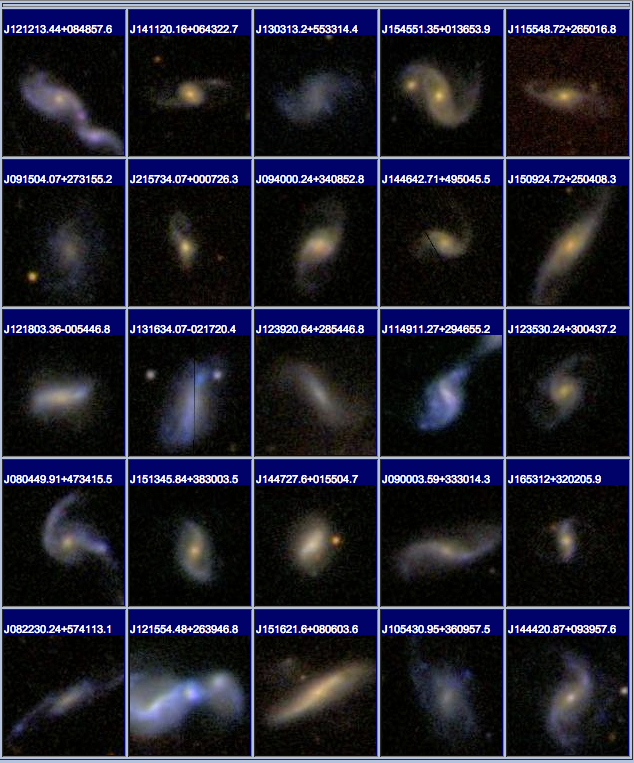
\includegraphics[angle=0,width=7.0in]{figures/gallery/loose.png}
\caption{Example $gri$ cutout images for galaxies identified as having ``loose'' winding spiral arms (Task 10, Answer 30) from the GZ2 clean, debiased sample. Format is the same as Figure~\ref{fig1}.}
\end{figure*}

\newpage
\clearpage
\begin{figure*}
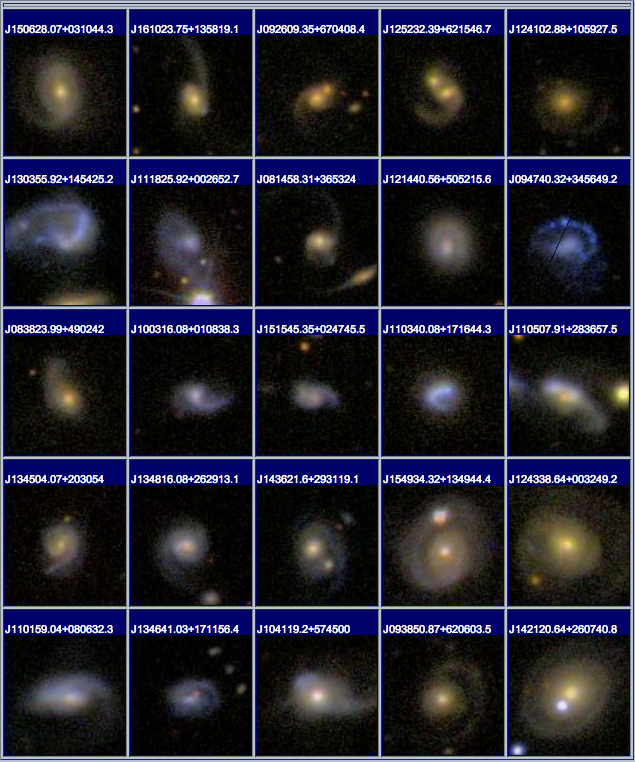
\includegraphics[angle=0,width=7.0in]{figures/gallery/spiral1.png}
\caption{Example $gri$ cutout images for galaxies identified as having 1 spiral arm (Task 11, Answer 31) from the GZ2 clean, debiased sample. Format is the same as Figure~\ref{fig1}.}
\end{figure*}

\newpage
\clearpage
\begin{figure*}
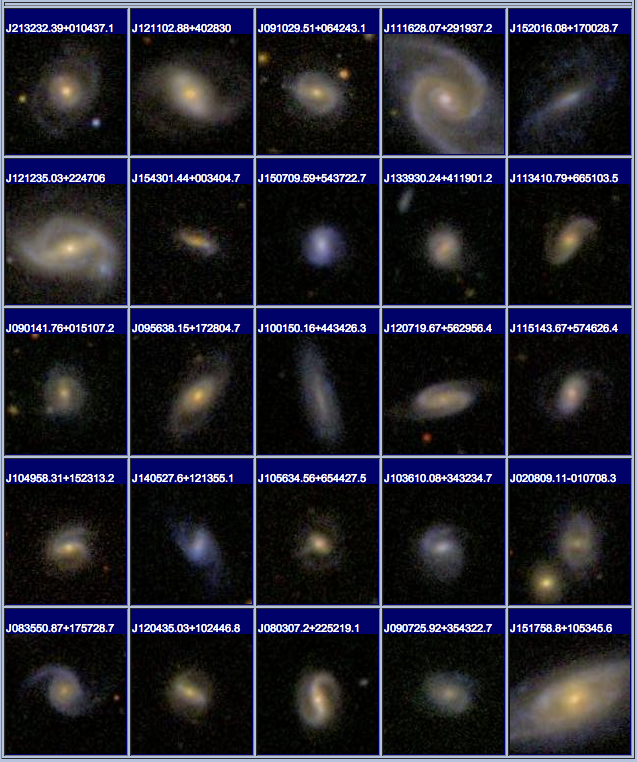
\includegraphics[angle=0,width=7.0in]{figures/gallery/spiral2.png}
\caption{Example $gri$ cutout images for galaxies identified as having 2 spiral arms (Task 11, Answer 32) from the GZ2 clean, debiased sample. Format is the same as Figure~\ref{fig1}.}
\end{figure*}

\newpage
\clearpage
\begin{figure*}
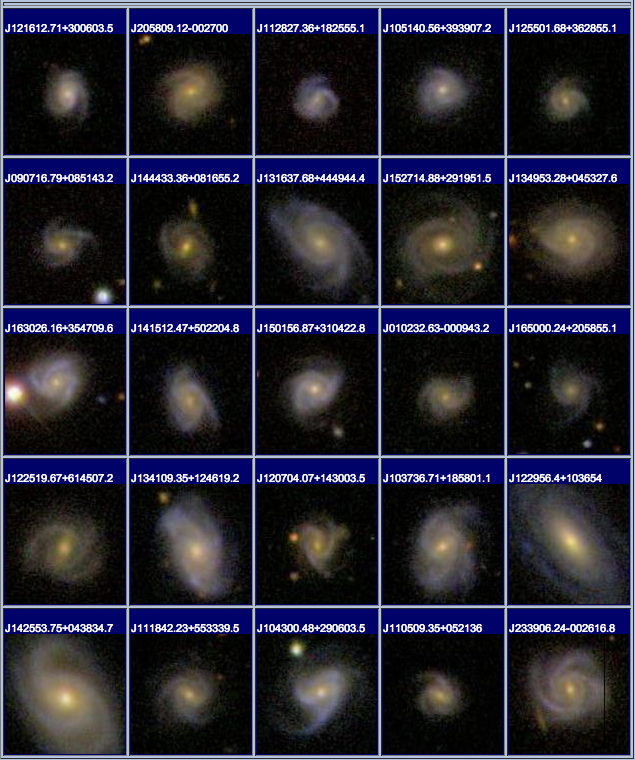
\includegraphics[angle=0,width=7.0in]{figures/gallery/spiral3.png}
\caption{Example $gri$ cutout images for galaxies identified as having 3 spiral arms (Task 11, Answer 33) from the GZ2 clean, debiased sample. Format is the same as Figure~\ref{fig1}.}
\end{figure*}

\newpage
\clearpage
\begin{figure*}
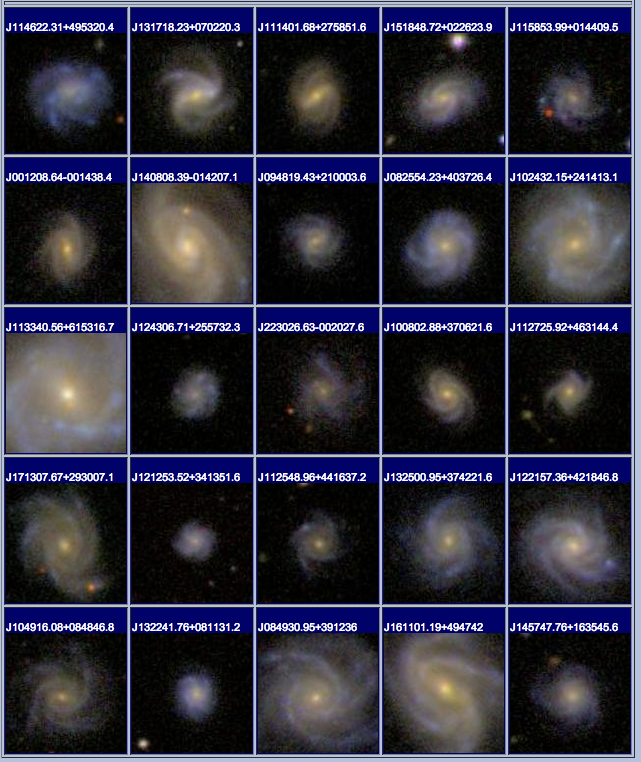
\includegraphics[angle=0,width=7.0in]{figures/gallery/spiral4.png}
\caption{Example $gri$ cutout images for galaxies identified as having 4 spiral arms (Task 11, Answer 34) from the GZ2 clean, debiased sample. Format is the same as Figure~\ref{fig1}.}
\end{figure*}

\newpage
\clearpage
\begin{figure*}
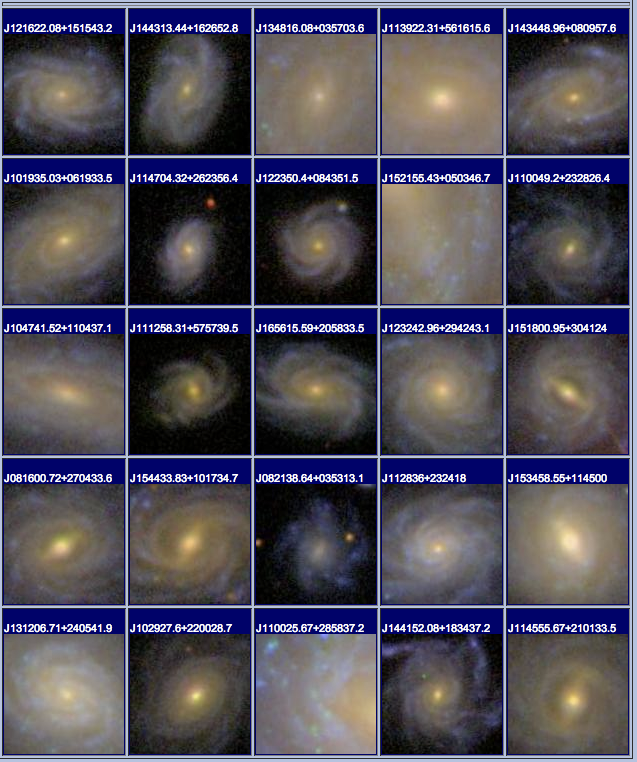
\includegraphics[angle=0,width=7.0in]{figures/gallery/spiralmorethan4.png}
\caption{Example $gri$ cutout images for galaxies identified as having more than 4 spiral arms (Task 11, Answer 36) from the GZ2 clean, debiased sample. Format is the same as Figure~\ref{fig1}.}
\end{figure*}

\newpage
\clearpage
\begin{figure*}
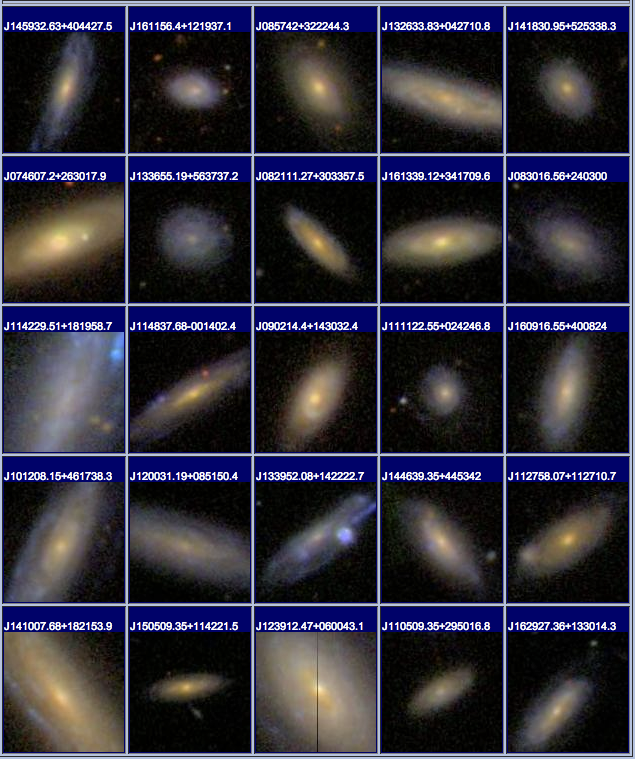
\includegraphics[angle=0,width=7.0in]{figures/gallery/spiralcanttell.png}
\caption{Example $gri$ cutout images for galaxies identified as spiral arms, but ``can't tell'' how many (Task 11, Answer 37) from the GZ2 clean, debiased sample. Format is the same as Figure~\ref{fig1}.}
\end{figure*}

\end{document}

